\documentclass[twocolumn,twoside,12pt]{article}

%\usepackage[spanish,activeacute]{babel}


\usepackage[colorlinks = true,
            linkcolor = blue,
            urlcolor  = blue,
            citecolor = blue,
            anchorcolor = blue]{hyperref}

\newcommand{\changeurlcolor}[1]{\hypersetup{urlcolor=#1}}  
\usepackage{textcomp}
\usepackage{anysize}
\marginsize{2cm}{2cm}{1.5cm}{1.5cm}
\newtheorem{theorem}{Teorema}
\usepackage{listings}
\lstset{language=Python} 
\usepackage{graphicx}
\usepackage{float}
%\graphicspath{ {c:/Users/MenTaLisT/Repositorios/Proyecto_BC/PDF/imagenes} }
\title{Herramienta para el an\'alisis de las prote\'inas que interact\'uan con LASP-1\\
 \begin{large} 
  Repositorio: \url{https://github.com/Fabio-Coronado/Proyecto_BC}
\end{large}}
\author{Fabio Coronado,  Rodrigo Paz }

\begin{document}

\maketitle


\begin{abstract}

The proposal for this project is to carry out a graphic interface that facilitates the analysis of the proteins that interact with LASP-1 and its association with different types of carcinomas, especially hepatocellular carcinoma related to HBV, in addition to carrying out a phylogenetic analysis of these proteins that It will allow us to locate its evolutionary origin.

For phylogenetic analysis we will look for their respective orthologs that will help us find the origin of these proteins.
\end{abstract}
\section{Resumen Ejecutivo}

La propuesta para este proyecto es realizar una interfaz gr\'afica que facilite el an\'alisis de las prote\'inas que interact\'uan con LASP-1 y su asociaci\'on con distintos tipos c\'arcinomas en especial el carcinoma hepatocelular relacionado con el VHB, adem\'as de
realizar un \'analisis filogen\'etico de estas prote\'inas que nos permitir\'a ubicar su origen evolutivo.

Para el an\'alisis filogen\'etico buscaremos sus respectivos ort\'ologos que nos ayudar\'an a encontrar el origen de estas prote\'inas.\\




\section{Descripci\'on del proyecto}

Para este proyecto se toma en cuenta un estudio realizado que est\'a mencionado en la bibliograf\'ia. El estudio realiza el siguiente an\'alisis:
\begin{itemize}
\item Para encontrar las prote\'inas que interactuan con LASP-1, se recoge informaci\'on de prote\'inas humanas en distintas base de datos. Una vez encontradas las prote\'inas se descartan las prote\'inas que no son validadas experimentalmente.
\item Luego se eval\'ua la clase de proteína de los interactuadores LASP-1 utilizando el sistema de clasificación PANTHER.
Se realiza la anotaci\'on de la funci\'on g\'enica de los interactuadores LASP-1 con el an\'alisis GO.
\item Las rutas en las que los interactores LASP-1 est\'an involucrados son evaluadas por la ruta KEGG y la ruta PANTHER, se construye la red de interacci\'on que contiene nodos correspondientes a LASP-1 con sus prote\'inas interactuantes y se integra a\'un m\'as la informaci\'on de interacci\'on de interactuadores LASP-1 con sus rutas asociadas.
\item Como se sabe de la sobreexpresi\'on de LASP-1 en HCC, y se asocia con infección por VHB en pacientes con CHC, se investig\'o si los interactuadores LASP-1 también están asociados con CHC relacionado con VHB.
\item Basado en el an\'alisis de perfiles de expresi\'on g\'enica de GSE14520, se encontr\'o que el cambio en LASP-1 fue mayor de 2.0 veces con un P-valve $<0.05$ en tejidos HBV-HCC en comparación con tejidos no HCC como se muestra en la Figura 1. 


\begin{figure}[H]
    \centering
    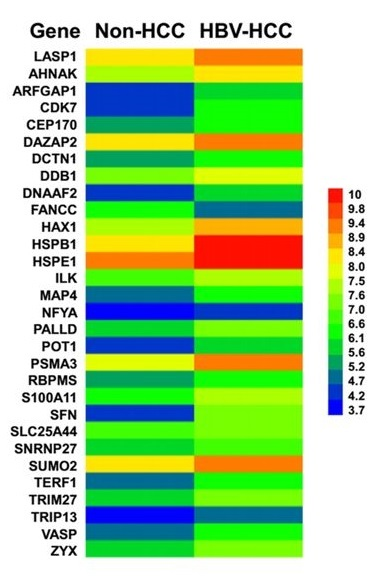
\includegraphics[scale=0.5]{imagenes/figura1.jpg}
    \caption{La expresi\'on relativa de los interactuadores LASP-1 con un cambio de pliegue de aproximadamente 2 y $P <0.05$}
    \label{fig:tabla}
\end{figure}

\item Entre estos genes, solo FANCC esta regulado negativamente en el HCC relacionado con el VHB, y los niveles de expresi\'on de otros 28 genes aumentaron en las c\'elulas enfermas.

\end{itemize}
Escogeremos las siguientes prote\'inas de las 28 que aumentaron su expresi\'on, estas ser\'an:
\begin{itemize}
\item LASP-1
\item ZYX
\item HSPB1
\item SFN
\item HAX1
\item SUMO2
\item ILK
\end{itemize}
Al realizar una investigaci\'on en distintas \'areas muchas veces el limitante  es el financiamiento,  para ayudar quitar costos hemos optado en este proyecto por crear un software que utiliza recursos gratuitos como librer\'ias de python para la parte bioinform\'atica en las que se incluir\'an : biopython, biopandas y para el GUI utilizaremos Tkinter.\\
Otro factor que puede ser limitante es el hardware disponible, por lo que en lugar de descargar las bases de datos, realizaremos consultas a las base de datos en l\'inea mediante el programa.\\

Las herramientas que ser\'an implementadas en el software (GUI) ser\'an: 
\begin{itemize}
 \item Alineamiento global de secuencias. 
 \item Alineamiento local de secuencias. 
 \item Alineamiento m\'ultiple de secuencias.
 \item Algoritmos de b\'usqueda de secuencias en Base de datos.
 \item Algoritmo BLASTp.
 \item Algotirmo para el an\'alisis filogen\'etico.
\end{itemize}

  
Se incluir\'an distintos algoritmos de programaci\'on dinamica: como los algoritmos de alineamiento de secuencias usando una matriz BLOSUM62 (puede ser cambiada), Algoritmo Blast para la b\'usqueda de secuencias similares en una base de datos, Algoritmo CLUSTALW para el alinemaiento m\'ultiple.  

Se entregar\'an los avances de acuerdo al siguiente cronograma:\\

\textbf{Entregable 1(Practica Calif N.2.:})
\begin{itemize}
\item Propuesta del Proyecto.\\
\end{itemize}


\textbf{Entregable 2(Práctica Calif N.3.):}
\begin{itemize}
\item Versi\'on final de la propuesta en PDF.
\item Prote\'inas escogidas que interact\'uan con LASP-1.
\item Avance del proyecto al 30\%.\\
\end{itemize}

\textbf{Entregable 3(Práctica Calif N.4.):}
\begin{itemize}
\item Implementaci\'on al 70\%.
\item C\'alculo de descriptores de interacci\'on prote\'ina - prote\'ina con el software.\\

\end{itemize}

\textbf{Entregable 4 (Lab. Calif. N.4):}
\begin{itemize}
\item Implementaci\'on al 100\%. Incluye: C\'odigo fuente, Librer\'ias, datos de
prueba, reporte final. (DVD o repositorio p\'ublico).
\item An\'alisis y Generaci\'on de \'Arboles Filogen\'eticos.\\


\end{itemize}

Aporte personal de cada integrante:\\
\begin{itemize}
\item Fabio Coronado:
      \begin{itemize}
    
      \item An\'alisis filogen\'etico.
      \item Algoritmos de b\'usqueda de secuencias en Base de datos.
      \item Alineamiento de secuencias. 
      \end{itemize}
\item Rodrigo Paz:
      \begin{itemize}
      \item Implementaci\'on del GUI en Tkinter.
      \item Algoritmo BLASTp.
      \item Alineamiento m\'ultiple de secuencias.
      \end{itemize}

\end{itemize}



\section{Algoritmos e Implementaci\'on Computacional}


En el proyecto se implement\'ran distintos algoritmos que tienen un costo computacional adecuado para el an\'alisis de una gran cantidad de datos.\\

Algunos algoritmo ya implementados para esta presentaci\'on:\\
\\

\textbf{Algoritmo de Needleman-Wunsch:}
\footnotesize
\begin{lstlisting}[frame=single]

def needleman_Wunsch(seq1,seq2,sm,g):
S = [[0]]
T = [[0]]
# initialize gaps row
for j in range(1, len (seq2)+1):
S[0].append(g * j)
T[0].append(3)
# initialize gaps column
for i in range(1, len (seq1)+1):
S.append([g * i])
T.append([2])
# apply the recurrence relation 
#to fill the remaining of the
#matrix
for i in range(0, len (seq1)):
for j in range( len (seq2)):

s1=S[i][j]+score_pos(seq1[i],seq2[j],sm,g);
s2 = S[i][j+1] + g
s3 = S[i+1][j] + g
S[i+1].append(max(s1, s2, s3))
T[i+1].append(max3t(s1, s2, s3))
return (S, T)
def max3t (v1, v2, v3):
if v1 > v2:
if v1 > v3: return 1
else : return 3
else :
if v2 > v3: return 2
else : return 3

\end{lstlisting}
\normalsize
\textbf{Algoritmo de Smith-Waterman:}
\footnotesize
\begin{lstlisting}[frame=single]

def smith_Waterman (seq1, seq2, sm, g):
S = [[0]]
T = [[0]]
maxscore = 0
for j in range(1, len (seq2)+1):
  S[0].append(0)
  T[0].append(0)
for i in range(1, len (seq1)+1):
  S.append([0])
  T.append([0])
for i in range(0, len (seq1)):
  for j in range( len (seq2)):
     s1 = S[i][j] + 
        score_pos(seq1[i], seq2[j], sm, g)
     s2 = S[i][j+1] + g
     s3 = S[i+1][j] + g
     b = max(s1, s2, s3)
     if b <= 0:
       S[i+1].append(0)
       T[i+1].append(0)
     else:
       S[i+1].append(b)
       T[i+1].append(max3t(s1, s2, s3))
       if b > maxscore:
          maxscore = b
return (S, T, maxscore)

\end{lstlisting}
\normalsize

\textbf{Algoritmo para obtener el alineamiento:} \\
 \small
\begin{lstlisting}[frame=single]
def recover_align (T, seq1, seq2):
res = ["", ""]
i = len (seq1)
j = len (seq2)
while i>0 or j>0:
i f T[i][j]==1:
res[0] = seq1[i-1] + res[0]
res[1] = seq2[j-1] + res[1]
i -= 1
j -= 1
e l i f T[i][j] == 3:
res[0] = "-" + res[0]
res[1] = seq2[j-1] + res[1]
j -= 1
e l s e :
res[0] = seq1[i-1] + res[0]
res[1] = "-" + res[1]
i -= 1
return res

\end{lstlisting}
\normalsize
\textbf{Alineamiento m\'ultiple de secuencias en Biopython:}
\scriptsize
\begin{lstlisting}[frame=single]
from Bio import Alphabet
from Bio.SeqRecord import SeqRecord
from Bio.Align import MultipleSeqAlignment
from Bio.Alphabet import IUPAC
from Bio.Seq import Seq
seq1="MHQAIFIYQIGYPLKSGYIQSIRSPEYDNW"
seq2="MH--IFIYQIGYALKSGYIQSIRSPEY-NW"
seq3="MHQAIFI-QIGYALKSGY-QSIRSPEYDNW"

seqr1=SeqRecord(Seq(seq1,
Alphabet.Gapped(IUPAC.protein)),id ="seq1")
seqr2=SeqRecord(Seq(seq2,
Alphabet.Gapped(IUPAC.protein)),id ="seq2")
seqr3=SeqRecord(Seq(seq3,
Alphabet.Gapped(IUPAC.protein)),id ="seq3")
 
alin=MultipleSeqAlignment([seqr1, seqr2, seqr3])
print(alin)

#diferentes formas de imprimir:
# 2nd sequence
print (alin[1]) 
# 3rd column
print (alin[:,2]) 
# 4th to 7th columns (all sequences)
print (alin[:,3:7]) 
# first 3 columns of seq1
print (alin[0].seq[:3]) 
# sequences 2 and 3; 4th to 10th column
print (alin[1:3,5:12]) 

\end{lstlisting}	
\normalsize

\textbf{Algoritmo para usar Blastp:}\\
\scriptsize
\begin{lstlisting}[frame=single]
from Bio.Blast import NCBIWWW
from Bio.Blast import NCBIXML
from Bio import SeqIO
import re
#guarda un archivo xml
def Blast(archivofasta, direccion
                       ,nombrearchivo):
    
record = SeqIO.read(open(archivofasta),
                           format="fasta")

result_handle = NCBIWWW.qblast("blastp",
                 "nr", record.format("fasta"))
save_file = open( direccion+"/"+
                    nombrearchivo+".xml", "w")
save_file.write(result_handle.read())
save_file.close()
result_handle.close()

\end{lstlisting}	

\normalsize
\section{Resultados}
\begin{itemize}
	\item Esperamos encontrar el origen evolutivo de las proteinas escogidas.
	    
    \item Adem\'as esperamos demostrar con el \'arbol filogen\'etico el origen de LASP-1, ya sabemos de antemano que algunos an\'alisis indican que puede tener origen en la evoluci\'on de invertebrados a vertebrados.	
    
\end{itemize}

\section{Conclusiones}

\begin{itemize}
\item En un futuro se podr\'ia implementar mas funcionalidades el software como: Modelamiento de proteinas con PyMol, Algoritmos ocultos de Markov, Motif Discovery, etc.
\item Conocer el origen evolutivo de estas prote\'inas nos permitir\'a estar m\'as cerca de encontrar el origen de  distintos tipo de c\'ancer, esto tal vez ayudar\'a a encontrar tratamientos m\'as efectivos.
\item Con el pasar del tiempo se descubren diferentes prote\'inas que interact\'uan con carcinomas, encontrar las prote\'inas correctas mejorar\'a el diagn\'ostico de los distintos tipos de c\'ancer.
\item Al ser una herramienta que incluye librer\'ias libres permite ahorrar costos en la investigaci\'on.  

\end{itemize}


\begin{thebibliography}{X}

	\bibitem{LaTeX}
	Kong Fan-Yun, Zhu Ting, Li Nan, Cai Yun-Fei,Zhou Kai,Wei Xiao, Kou Yan-Bo, You Hong-Juan, Zheng   
	Kui-Yang,Tang Ren-Xian\\
\newblock {\em  Analysis of the proteins interacting with LASP-1 and their association with HBV-related hepatocellular carcinoma},
\newblock 03 March 2017,\\
\url{https://www.nature.com/articles/srep44017}

	\bibitem{LaTeX}
	Alan D. Moore.\\
\newblock {\em  Python GUI Programming with Tkinter},
\newblock May 2018

    
	\bibitem{LaTeX}
	Miguel Rocha , Pedro G. Ferreira.\\
\newblock {\em Bioinformatics Algorithms, Design and Implementation in Python},
\newblock 2018
	
	
	\bibitem{LaTeX}
   Tiago Antao.\\
\newblock {\em   Bioinformatics with Python Cookbook - Second Edition},
\newblock 2018


	
\end{thebibliography}


\end{document}